\documentclass[10pt]{beamer}

% Packages
\usepackage[utf8]{inputenc}
\usepackage[T1]{fontenc}
\usepackage{amsmath, amssymb, amsthm}
\usepackage{graphicx}
\usepackage{booktabs}
\usepackage{hyperref}
\usepackage{tikz}
\usetikzlibrary{shapes,arrows,positioning}

% Theme settings
\usetheme{default}
\usecolortheme{default}
\usefonttheme{professionalfonts}

\definecolor{ImperialBlue}{RGB}{0, 62, 116}
\definecolor{DarkGray}{RGB}{51, 51, 51}
\definecolor{LightGray}{RGB}{245, 245, 245}
\definecolor{AccentOrange}{RGB}{214, 96, 77}
\definecolor{AccentGreen}{RGB}{46, 139, 87}

% Apply colors
\setbeamercolor{frametitle}{fg=ImperialBlue, bg=white}
\setbeamercolor{title}{fg=ImperialBlue}
\setbeamercolor{structure}{fg=ImperialBlue}
\setbeamercolor{normal text}{fg=DarkGray}
\setbeamercolor{block title}{fg=white, bg=ImperialBlue}
\setbeamercolor{block body}{fg=DarkGray, bg=LightGray}
\setbeamercolor{itemize item}{fg=ImperialBlue}
\setbeamercolor{enumerate item}{fg=ImperialBlue}

% Remove navigation symbols
\setbeamertemplate{navigation symbols}{}

% Customize frame title
\setbeamertemplate{frametitle}{
  \vspace{0.5em}
  \insertframetitle
  \vspace{0.3em}
}

% Customize itemize
\setbeamertemplate{itemize items}[circle]
\setlength{\leftmargini}{1.5em}

% Footer
\setbeamertemplate{footline}{
  \leavevmode%
  \hbox{%
  \begin{beamercolorbox}[wd=.333333\paperwidth,ht=2.25ex,dp=1ex,left]{author in head/foot}%
    \hspace{1em}\usebeamerfont{author in head/foot}\insertshortauthor
  \end{beamercolorbox}%
  \begin{beamercolorbox}[wd=.333333\paperwidth,ht=2.25ex,dp=1ex,center]{title in head/foot}%
    \usebeamerfont{title in head/foot}\insertshorttitle
  \end{beamercolorbox}%
  \begin{beamercolorbox}[wd=.333333\paperwidth,ht=2.25ex,dp=1ex,right]{date in head/foot}%
    \usebeamerfont{date in head/foot}\insertshortdate{}\hspace*{2em}
    \insertframenumber{} / \inserttotalframenumber\hspace*{2ex} 
  \end{beamercolorbox}}%
  \vskip0pt%
}

% Title page customization
\setbeamertemplate{title page}{
  \vbox{}
  \vfill
  \begingroup
    \centering
    {\usebeamercolor[fg]{title}\usebeamerfont{title}\inserttitle\par}
    \vskip0.5em
    {\usebeamercolor[fg]{subtitle}\usebeamerfont{subtitle}\insertsubtitle\par}
    \vskip2em
    {\usebeamercolor[fg]{author}\usebeamerfont{author}\insertauthor\par}
    \vskip0.5em
    {\usebeamercolor[fg]{institute}\usebeamerfont{institute}\insertinstitute\par}
    \vskip1em
    {\usebeamercolor[fg]{date}\usebeamerfont{date}\insertdate\par}
  \endgroup
  \vfill
}

% Commands for highlighting
\newcommand{\emphbox}[1]{\colorbox{LightGray}{\textcolor{DarkGray}{#1}}}
\newcommand{\highlight}[1]{\textcolor{AccentOrange}{\textbf{#1}}}
\newcommand{\good}[1]{\textcolor{AccentGreen}{#1}}
\newcommand{\bad}[1]{\textcolor{AccentOrange}{#1}}

%----------------------------------------------------------------------------------------
\title{Smart Contracts and Decentralised Applications}
\subtitle{ECOM215: Blockchain Economics and Digital Assets}
\author{Dr Daniele Bianchi}
\institute{Queen Mary, University of London}
\date{Semester B, 2025/2026}
%----------------------------------------------------------------------------------------

\begin{document}

\AtBeginSection[]{
  \begin{frame}[plain]
    \vfill
    \begin{center}
      {\Large\color{ImperialBlue}\insertsection}
    \end{center}
    \vfill
  \end{frame}
}

\begin{frame}[plain]
  \titlepage
\end{frame}

\begin{frame}{Today's Agenda}
  \tableofcontents
\end{frame}

%----------------------------------------------------------------------------------------
\section{From Value Transfer to Programmable Money}
%----------------------------------------------------------------------------------------

\begin{frame}{Bitcoin vs Ethereum: A Key Distinction}
  \textbf{Bitcoin} (2009): Digital cash
  \begin{itemize}
    \item Transfers value from A to B
    \item Limited scripting: ``If condition X, then pay Y''
    \item Designed for one purpose: peer-to-peer payments
  \end{itemize}
  
  \vspace{1em}
  \textbf{Ethereum} (2015): Programmable platform
  \begin{itemize}
    \item Executes arbitrary programs on the blockchain
    \item Programs can hold funds, enforce rules, interact with each other
    \item Designed as a general-purpose ``world computer''
  \end{itemize}
  
  \vspace{1em}
  \textbf{The key insight}: What if we could program \textit{any} financial agreement to execute automatically, without relying on intermediaries to enforce it?
\end{frame}

\begin{frame}{A Motivating Example: Escrow}
  \textbf{The problem}: Alice wants to buy a laptop from Bob online. Neither trusts the other.
  
  \vspace{1em}
  \textbf{Traditional solution}: Use an escrow service (PayPal, bank, lawyer)
  \begin{itemize}
    \item Alice pays the escrow agent
    \item Bob ships the laptop
    \item Alice confirms receipt; escrow releases funds to Bob
    \item If dispute: escrow arbitrates
  \end{itemize}
  
  \vspace{0.5em}
  \bad{Problem}: The escrow agent charges fees, can make errors, might be unavailable, and must be trusted.
  
  \vspace{1em}
  \textbf{Smart contract solution}:
  \begin{itemize}
    \item A program holds Alice's funds
    \item When both parties confirm (or a timeout expires), funds release automatically
    \item Rules are public, execution is guaranteed, no middleman
  \end{itemize}
\end{frame}

\begin{frame}{What Makes Ethereum Different}
  Ethereum introduced the \highlight{Ethereum Virtual Machine} (EVM)---a global, decentralised computer that executes programs called \textit{smart contracts}.
  
  \vspace{1em}
  \begin{center}
  \begin{tabular}{lcc}
    \toprule
    & \textbf{Bitcoin} & \textbf{Ethereum} \\
    \midrule
    Primary purpose & Value transfer & Programmable applications \\
    Native currency & BTC & ETH \\
    Scripting & Limited & General-purpose \\
    Programs on-chain & No & Yes (smart contracts) \\
    Consensus (2024) & Proof-of-Work & Proof-of-Stake \\
    \bottomrule
  \end{tabular}
  \end{center}
  
  \vspace{1em}
  ETH serves two purposes: (1) a store of value like BTC, and (2) \highlight{``fuel''} to pay for computation on the network.
\end{frame}

%----------------------------------------------------------------------------------------
\section{What is a Smart Contract?}
%----------------------------------------------------------------------------------------

\begin{frame}{Smart Contracts: Definition}
  \begin{block}{Definition}
    A \textbf{smart contract} is a program stored on a blockchain that automatically executes when predetermined conditions are met.
  \end{block}
  
  \vspace{1em}
  Think of it like a \highlight{vending machine}:
  \begin{itemize}
    \item Rules are fixed and visible (insert \$2, select item)
    \item Execution is automatic (machine dispenses item)
    \item No negotiation, no discretion, no human involvement
    \item Once deployed, the machine behaves the same way for everyone
  \end{itemize}
  
  \vspace{1em}
  A smart contract is similar: the rules are written in code, and the blockchain guarantees that the rules execute exactly as written.
\end{frame}

\begin{frame}{The ``Contract'' Misnomer}
  \textbf{Important clarification}: Smart contracts are \highlight{not legal contracts}.
  
  \vspace{1em}
  \begin{itemize}
    \item They don't have legal standing (in most jurisdictions)
    \item They can't understand intent or context
    \item They execute exactly what the code says---even if that's not what anyone wanted
  \end{itemize}
  
  \vspace{1em}
  Better mental model: Smart contracts are \textbf{autonomous agents} or \textbf{self-executing programs}.
  
  \vspace{1em}
  \textbf{The term's origin}: Nick Szabo coined ``smart contract'' in 1994 to describe agreements embedded in hardware/software. The blockchain implementation is more limited than his original vision.
\end{frame}

\begin{frame}{Key Properties of Smart Contracts}
  \textbf{1. Immutable}: Once deployed, the code cannot be changed.
  \begin{itemize}
    \item This is a feature (predictability) and a bug (can't fix errors)
  \end{itemize}
  
  \vspace{0.5em}
  \textbf{2. Deterministic}: Given the same inputs, always produces the same outputs.
  \begin{itemize}
    \item Every node that runs the contract gets the same result
  \end{itemize}
  
  \vspace{0.5em}
  \textbf{3. Atomic}: Transactions either fully complete or fully fail.
  \begin{itemize}
    \item No partial execution---prevents inconsistent states
  \end{itemize}
  
  \vspace{0.5em}
  \textbf{4. Transparent}: Anyone can inspect the code and its execution history.
  \begin{itemize}
    \item Enables auditing, but also reveals vulnerabilities to attackers
  \end{itemize}
  
  \vspace{0.5em}
  \textbf{5. Permissionless}: Anyone can deploy or interact with contracts.
  \begin{itemize}
    \item No approval needed, but no recourse if something goes wrong
  \end{itemize}
\end{frame}

\begin{frame}{What Can Smart Contracts Do?}
  Smart contracts can:
  
  \vspace{0.5em}
  \begin{itemize}
    \item \good{Hold and transfer cryptocurrency}
    \item \good{Enforce rules automatically} (e.g., release payment when condition met)
    \item \good{Create and manage tokens} (ERC-20, NFTs)
    \item \good{Interact with other contracts} (composability)
    \item \good{Record data immutably}
  \end{itemize}
  
  \vspace{1em}
  Smart contracts \textbf{cannot}:
  
  \vspace{0.5em}
  \begin{itemize}
    \item \bad{Access external data directly} (need oracles---more on this later)
    \item \bad{Initiate actions on their own} (must be triggered by a transaction)
    \item \bad{Be modified after deployment} (except through upgrade patterns)
    \item \bad{Understand intent} (only execute literal code)
  \end{itemize}
\end{frame}

%----------------------------------------------------------------------------------------
\section{How Smart Contracts Work}
%----------------------------------------------------------------------------------------

\begin{frame}{The Lifecycle of a Smart Contract}
  \textbf{Step 1: Development}
  \begin{itemize}
    \item Developer writes code in a high-level language (e.g., Solidity)
    \item Code is compiled into bytecode the EVM can execute
  \end{itemize}
  
  \vspace{0.5em}
  \textbf{Step 2: Deployment}
  \begin{itemize}
    \item A special transaction publishes the bytecode to the blockchain
    \item The contract receives a unique address (like an account)
    \item Deployment costs gas (more complex contracts cost more)
  \end{itemize}
  
  \vspace{0.5em}
  \textbf{Step 3: Interaction}
  \begin{itemize}
    \item Users send transactions to the contract address
    \item Each transaction specifies which function to call and with what inputs
    \item The contract executes and updates its state
  \end{itemize}
  
  \vspace{0.5em}
  \textbf{Step 4: State changes are recorded}
  \begin{itemize}
    \item Results are written to the blockchain permanently
  \end{itemize}
\end{frame}

\begin{frame}{A Simple Example: Payment Splitter}
  Imagine a contract that automatically splits incoming payments 50/50 between two addresses.
  
  \vspace{1em}
  \textbf{What the contract stores}:
  \begin{itemize}
    \item Address A (first recipient)
    \item Address B (second recipient)
  \end{itemize}
  
  \vspace{0.5em}
  \textbf{What the contract does}:
  \begin{itemize}
    \item When ETH is sent to the contract, automatically forward 50\% to A and 50\% to B
  \end{itemize}
  
  \vspace{1em}
  \textbf{Key point}: Once deployed, this contract will \textit{always} split payments 50/50. The developer cannot change the split. The recipients cannot stop it. No one can redirect the funds elsewhere.
  
  \vspace{0.5em}
  This is both the power and the danger of smart contracts.
\end{frame}

\begin{frame}{The Ethereum Virtual Machine (EVM)}
  Every Ethereum node runs the same virtual machine---the \highlight{EVM}.
  
  \vspace{1em}
  \textbf{What you need to know}:
  \begin{itemize}
    \item The EVM executes smart contract code
    \item Every node runs the same code and must get the same result
    \item This is how the network reaches consensus on contract outcomes
  \end{itemize}
  
  \vspace{1em}
  \textbf{Why this matters economically}:
  \begin{itemize}
    \item Computation is replicated across thousands of nodes
    \item This is intentionally inefficient (that's the cost of trustlessness)
    \item Users must pay for this computation---hence \highlight{gas fees}
  \end{itemize}
  
  \vspace{1em}
  The EVM is the ``engine'' that makes programmable money possible, but its inefficiency is why fees can be high during congestion.
\end{frame}

%----------------------------------------------------------------------------------------
\section{Gas and Transaction Fees}
%----------------------------------------------------------------------------------------

\begin{frame}{Why Gas Exists}
  \textbf{The problem}: If computation is free, attackers could deploy infinite loops that freeze the network.
  
  \vspace{1em}
  \textbf{The solution}: Make users pay for every computational step.
  
  \vspace{1em}
  \begin{block}{Gas}
    A unit measuring computational work. Every operation has a gas cost. Users pay for the gas their transactions consume.
  \end{block}
  
  \vspace{0.5em}
  \textbf{Examples}:
  \begin{itemize}
    \item Simple ETH transfer: 21,000 gas
    \item Token transfer: $\approx$65,000 gas
    \item Complex DeFi transaction: 200,000+ gas
  \end{itemize}
  
  \vspace{1em}
  Gas serves two purposes: (1) prevents spam/abuse, and (2) compensates validators for processing transactions.
\end{frame}

\begin{frame}{How Fees Are Calculated}
  Since August 2021 (\highlight{EIP-1559}), Ethereum fees have two components:
  
  \vspace{1em}
  \textbf{Total fee} = Gas used $\times$ (Base fee + Priority fee)
  
  \vspace{1em}
  \begin{itemize}
    \item \textbf{Base fee}: Set by the protocol based on network congestion
    \begin{itemize}
      \item Increases when blocks are full, decreases when blocks have space
      \item This portion is \highlight{burned} (destroyed), reducing ETH supply
    \end{itemize}
    
    \vspace{0.5em}
    \item \textbf{Priority fee} (``tip''): Set by the user
    \begin{itemize}
      \item Higher tip = faster inclusion
      \item This portion goes to the validator
    \end{itemize}
  \end{itemize}

\vspace{1em}
\textbf{Example}: A simple ETH transfer requires 21,000 gas.
\begin{itemize}
  \item Base fee: 20 gwei per unit of gas (1 gwei = 0.000000001 ETH, one billionth)
  \item Priority fee (tip): 2 gwei per unit of gas
  \item Total fee: 21,000 $\times$ (20 + 2) = 462,000 gwei = 0.000462 ETH
\end{itemize}
\end{frame}

\begin{frame}{Gas Limit: Bounding Computation}
  Users also set a \highlight{gas limit}---the maximum gas they're willing to spend.
  
  \vspace{1em}
  \textbf{Why this matters}:
  \begin{itemize}
    \item If execution exceeds the gas limit, the transaction fails
    \item You still pay for the gas consumed up to that point
    \item Protects users from unexpectedly expensive transactions
  \end{itemize}
  
  \vspace{1em}
  \textbf{The block gas limit}:
  \begin{itemize}
    \item Each block has a maximum total gas ($\approx$30 million currently)
    \item This limits how much computation can happen per block
    \item It's why Ethereum can only process $\approx$15 transactions/second on L1
  \end{itemize}
  
  \vspace{1em}
  Gas limits are the mechanism that makes Ethereum ``quasi-Turing-complete''---it can run any program, but only up to a bounded amount of computation.
\end{frame}

\begin{frame}{Fee Dynamics in Practice}
  \begin{figure}
    \centering
    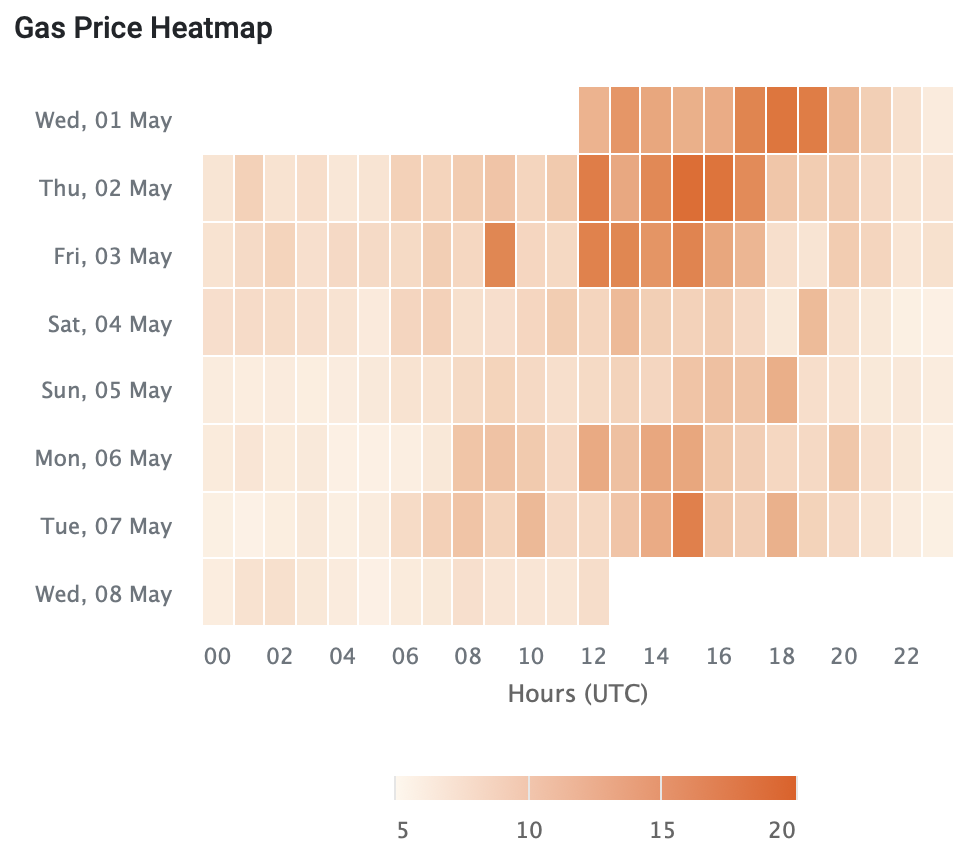
\includegraphics[width=.7\textwidth]{Figures/Gas price.png}
    \begin{flushleft}
      \footnotesize\textbf{Figure:} \normalfont Intra-day gas prices from 1--8 May 2024. Source: \url{etherscan.io}.
    \end{flushleft}
    \label{fig:gas}
  \end{figure}
\end{frame}


\begin{frame}{Fee Dynamics in Practice}
  
  \textbf{Fees vary dramatically based on market activity}:
  \begin{itemize}
    \item During low activity: A simple transfer might cost \$0.50
    \item During NFT mints or market crashes: The same transfer might cost \$50+
  \end{itemize}
  
  \vspace{1em}
  \textbf{Economic implications}:
  \begin{itemize}
    \item High fees price out small transactions
    \item Users compete for block space through tips
    \item Validators are incentivised to include highest-paying transactions
    \item Layer 2 solutions (Topic 2) offer lower fees by batching transactions
  \end{itemize}
  
  \vspace{1em}
  \textbf{EIP-1559's impact}: Base fee burning has made ETH supply dynamics complex---during high activity, more ETH is burned than issued, making ETH temporarily deflationary.
\end{frame}

%----------------------------------------------------------------------------------------
\section{The Limits of Smart Contracts}
%----------------------------------------------------------------------------------------

\begin{frame}{The Oracle Problem}
  \begin{block}{The Problem}
    Smart contracts can only access data stored on the blockchain. They cannot directly access real-world information.
  \end{block}
  
  \vspace{1em}
  \textbf{Examples of data contracts might need}:
  \begin{itemize}
    \item Asset prices (for DeFi)
    \item Weather data (for insurance)
    \item Sports scores (for betting)
    \item Shipment delivery confirmation (for trade finance)
  \end{itemize}
  
  \vspace{1em}
  \textbf{Solution}: \highlight{Oracles}---services feeding external data to smart contracts.
  
  \vspace{0.5em}
  \textbf{The catch}: Oracles reintroduce trust. If an oracle lies or fails, the contract executes on false data. The contract itself is trustless, but \textit{the system} depends on trusting the oracle.
  
  \vspace{0.5em}
  We'll explore oracles further in Topic 4 (DeFi), where they're critical infrastructure.
\end{frame}

\begin{frame}{``Code is Law''---And Its Consequences}
  Smart contracts execute exactly as written, \textit{even if that's not what anyone intended}.
  
  \vspace{1em}
  \textbf{Implications}:
  \begin{itemize}
    \item Bugs cannot be patched after deployment
    \item Exploits are ``legitimate'' from the blockchain's perspective
    \item There's no court to appeal to, no fraud protection
    \item Lost funds are usually gone forever
  \end{itemize}
  
  \vspace{1em}
  \textbf{This is a philosophical stance}, not just a technical limitation:
  \begin{itemize}
    \item Proponents: The whole point is removing human discretion
    \item Critics: Rigid code can't handle edge cases, mistakes, or malice
  \end{itemize}
  
  \vspace{1em}
  The tension between ``code is law'' and practical reality has led to contentious debates---including the one we'll discuss next.
\end{frame}

\begin{frame}{Case Study: The DAO Hack (2016)}
  \textbf{The DAO}: A decentralised investment fund on Ethereum. Raised \$150 million in ETH.
  
  \vspace{1em}
  \textbf{The exploit}: A \highlight{reentrancy bug} allowed an attacker to repeatedly withdraw funds before the contract updated its balance.
  
  \vspace{0.5em}
  \begin{itemize}
    \item The attacker drained 3.6 million ETH ($\approx$\$60 million at the time)
    \item The attack was ``legal'' by the contract's code
    \item From the blockchain's perspective, it was just a series of valid transactions
  \end{itemize}
  
  \vspace{1em}
  \textbf{The response}: The Ethereum community voted to ``hard fork''---rewrite history to return the stolen funds.
  
  \vspace{0.5em}
  \textbf{The controversy}:
  \begin{itemize}
    \item Supporters: Theft is theft; we should fix it
    \item Opponents: If we rewrite history once, Ethereum isn't immutable
    \item Result: Ethereum forked; opponents continued as ``Ethereum Classic''
  \end{itemize}
\end{frame}

\begin{frame}{Smart Contract Security Risks}
  The DAO wasn't unique. Common vulnerabilities include:
  
  \vspace{.5em}
  \begin{center}
  \begin{tabular}{lp{6.5cm}}
    \toprule
    \textbf{Vulnerability} & \textbf{What Happens} \\
    \midrule
    Reentrancy & Attacker calls back into contract before state updates \\
    Integer overflow & Numbers wrap around, enabling theft \\
    Access control & Unauthorised users can call restricted functions \\
    Oracle manipulation & Attacker feeds false price data \\
    Flash loan attacks & Borrow millions, manipulate market, repay in one transaction \\
    \bottomrule
  \end{tabular}
  \end{center}
  
  \vspace{1em}
  \textbf{Scale of the problem}: Billions of dollars have been lost to smart contract exploits. In 2022 alone, over \$3 billion was stolen from DeFi protocols.
  
  \vspace{0.5em}
  Security audits help but don't guarantee safety. Code complexity makes exhaustive verification difficult.
\end{frame}

%----------------------------------------------------------------------------------------
\section{Decentralised Applications (DApps)}
%----------------------------------------------------------------------------------------

\begin{frame}{What is a DApp?}
  \begin{block}{Definition}
    A \textbf{Decentralised Application} (DApp) is an application with its backend logic running on smart contracts rather than centralised servers.
  \end{block}
  
  \vspace{1em}
  \textbf{Typical architecture}:
  \begin{itemize}
    \item \textbf{Frontend}: Standard web/mobile interface (React, etc.)
    \item \textbf{Backend}: Smart contracts on Ethereum (or other blockchains)
    \item \textbf{Wallet}: User's wallet (e.g., MetaMask) signs transactions
  \end{itemize}
  
  \vspace{1em}
  \textbf{Key difference from traditional apps}:
  \begin{itemize}
    \item No company controls the backend
    \item Users interact directly with smart contracts
    \item Data and logic are publicly auditable
  \end{itemize}
\end{frame}

\begin{frame}{Benefits of DApps}
  \good{Zero downtime}: Smart contracts run as long as the blockchain exists---no server outages.
  
  \vspace{0.5em}
  \good{Censorship resistance}: No single entity can block users or shut down the application.
  
  \vspace{0.5em}
  \good{Transparency}: Code is public; anyone can verify what the application does.
  
  \vspace{0.5em}
  \good{Trustless operation}: Users don't need to trust the developer---they can verify the code.
  
  \vspace{0.5em}
  \good{Composability}: DApps can interact with each other, creating building blocks for complex systems (``money legos'').
  
  \vspace{1em}
  \textbf{Important caveat}: These benefits apply only to the on-chain components. Most DApps have off-chain elements (frontends, APIs) that remain centralised.
\end{frame}

\begin{frame}{Drawbacks of DApps}
  \bad{User experience}: Managing wallets, signing transactions, paying gas---all friction for mainstream users.
  
  \vspace{0.5em}
  \bad{Performance}: Blockchain is slow compared to centralised servers. Every state change requires consensus.
  
  \vspace{0.5em}
  \bad{Cost}: Users pay gas for every interaction. During congestion, simple actions can cost tens of dollars.
  
  \vspace{0.5em}
  \bad{Immutability}: Bugs can't be easily fixed. Data can't be deleted (privacy implications).
  
  \vspace{0.5em}
  \bad{Hidden centralisation}: Many DApps have centralised frontends, admin keys, or upgradeable contracts---undermining the ``decentralised'' label.
  
  \vspace{1em}
  \textbf{Reality check}: For most use cases, centralised applications are faster, cheaper, and easier. DApps make sense when trustlessness or censorship resistance are genuinely valuable.
\end{frame}

\begin{frame}{DApp Ecosystem: Examples}
  \textbf{Decentralised Finance (DeFi)}---Topic 4:
  \begin{itemize}
    \item Uniswap: Decentralised exchange
    \item Aave, Compound: Lending and borrowing
    \item MakerDAO: Stablecoin issuance
  \end{itemize}
  
  \vspace{0.5em}
  \textbf{NFTs and Digital Ownership}---Topic 7:
  \begin{itemize}
    \item OpenSea: NFT marketplace
    \item ENS: Decentralised domain names
  \end{itemize}
  
  \vspace{0.5em}
  \textbf{Infrastructure}:
  \begin{itemize}
    \item Chainlink: Oracle network
    \item The Graph: Indexing protocol
  \end{itemize}
  
  \vspace{0.5em}
  We'll explore DeFi applications in depth in Topic 4.
\end{frame}

%----------------------------------------------------------------------------------------
\section{Summary and Next Steps}
%----------------------------------------------------------------------------------------

\begin{frame}{Key Takeaways}
  \begin{enumerate}
    \item \textbf{Smart contracts are programs that execute automatically on the blockchain}
    \begin{itemize}
      \item Immutable, deterministic, atomic, transparent
    \end{itemize}
    
    \vspace{0.3em}
    \item \textbf{Ethereum's EVM enables programmable money}
    \begin{itemize}
      \item But computation is expensive and slow (by design)
    \end{itemize}
    
    \vspace{0.3em}
    \item \textbf{Gas fees pay for computation and prevent abuse}
    \begin{itemize}
      \item EIP-1559: Base fee (burned) + priority fee (to validator)
    \end{itemize}
    
    \vspace{0.3em}
    \item \textbf{Smart contracts have fundamental limitations}
    \begin{itemize}
      \item Oracle problem: Can't access external data directly
      \item Security risks: Bugs are permanent, exploits are costly
    \end{itemize}
    
    \vspace{0.3em}
    \item \textbf{DApps offer trustlessness but sacrifice UX and efficiency}
    \begin{itemize}
      \item Valuable when censorship resistance matters
    \end{itemize}
  \end{enumerate}
\end{frame}

\begin{frame}{What's Next}
  \textbf{Topic 4: Decentralised Finance (DeFi)}
  \begin{itemize}
    \item Automated Market Makers (Uniswap)
    \item Lending protocols (Aave, Compound)
    \item Stablecoins
    \item Oracles in practice (Chainlink)
    \item Yield farming and risks
  \end{itemize}
  
  \vspace{1em}
  \textbf{Preparation}:
  \begin{itemize}
    \item Think about: How could you create a market without a traditional market maker?
    \item Explore: Look at a DeFi protocol on DeFiLlama (defillama.com)---what metrics are tracked?
  \end{itemize}
\end{frame}

\begin{frame}[plain]
  \vfill
  \begin{center}
    {\Large Questions?}
  \end{center}
  \vfill
\end{frame}

\end{document}